\documentclass{standalone}
\usepackage{pgfplots}
\pgfplotsset{compat=newest}
\usepackage{amsmath}
\usepackage{siunitx}
\sisetup{round-mode=places,round-precision=1}

\begin{document}

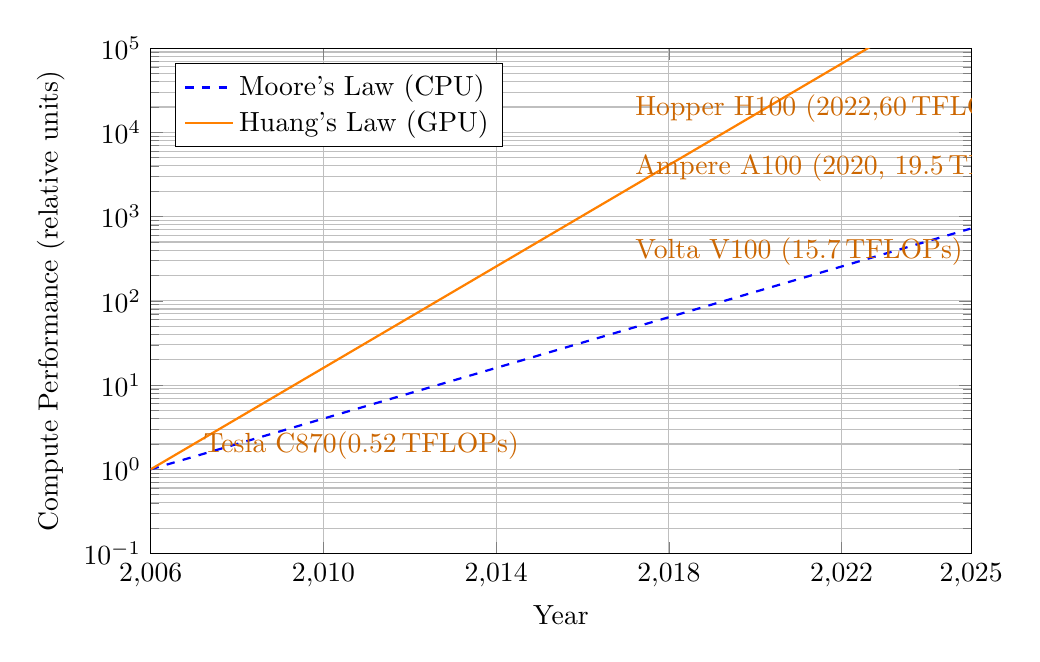
\begin{tikzpicture}
  \begin{semilogyaxis}[
    width=12cm, height=8cm,
    xlabel={Year},
    ylabel={Compute Performance (relative units)},
    xmin=2006, xmax=2025,
    ymin=0.1, ymax=1e5,
    xtick={2006,2010,2014,2018,2022,2025},
    grid=both,
    legend pos=north west,
    legend cell align=left,
    every axis plot/.append style={thick}
  ]

  % Moore's Law (doubling every two years)
  \addplot[
    blue, dashed, domain=2006:2025, samples=200
  ] {2^((x-2006)/2)};
  \addlegendentry{Moore's Law (CPU)}

  % Huang's Law (doubling every year)
  \addplot[
    orange, domain=2006:2025, samples=200
  ] {2^(x-2006)};
  \addlegendentry{Huang's Law (GPU)}

  % GPU Milestones
  \node[anchor=south west,orange!80!black] at (axis cs:2007,1) {Tesla C870(\SI{0.52}{TFLOPs})};
  \node[anchor=south west,orange!80!black] at (axis cs:2017,200) {Volta V100 (\SI{15.7}{TFLOPs})};
  \node[anchor=south west,orange!80!black] at (axis cs:2017,2000) {Ampere A100 (2020, \SI{19.5}{TFLOPs})};
  \node[anchor=south west,orange!80!black] at (axis cs:2017,10000) {Hopper H100 (2022,\SI{60}{TFLOPs})};
  \end{semilogyaxis}
\end{tikzpicture}

\end{document}
\begin{tikzpicture}
  %------------------ AXIS ------------------%
  \begin{semilogyaxis}[
    width=13.5cm, height=8.5cm,
    xlabel={Year}, ylabel={Compute Performance (TFLOPs, FP32 peak)},
    xmin=2006, xmax=2025,
    ymin=0.2, ymax=1e2,
    xtick={2006,2008,2010,2012,2014,2016,2018,2020,2022,2025},
    grid=both,
    legend pos=north west,
    legend cell align=left,
    tick align=outside,
    every axis plot/.append style={thick},
  ]

  %------------------ THEORETICAL TRENDS ------------------%
  % Moore's Law: ~2x every 2 years; normalized to 0.5 TFLOP at 2006 for visual match
  \addplot[blue, dashed, domain=2006:2025, samples=200]
    {0.5 * 2^((x-2006)/2)};
  \addlegendentry{Moore's Law (CPU, $\times 2$ / 2 yrs)}

  % Huang's Law: ~2x every year; normalized to 0.5 TFLOP at 2006
  \addplot[orange, domain=2006:2025, samples=200]
    {0.5 * 2^(x-2006)};
  \addlegendentry{Huang's Law (GPU, $\times 2$ / yr)}

  %------------------ DATA-DRIVEN GPU MILESTONES ------------------%
  % Year, TFLOPs, Label
  \addplot[
    only marks, mark=*,
    mark size=2.2pt, orange!85!black
  ] table[row sep=\\]{
    x     y
    2007  0.52   % Tesla C870 (approx FP32)
    2017  15.7   % Volta V100 (FP32 peak)
    2020  19.5   % Ampere A100 (FP32 peak)
    2022  60     % Hopper H100 (FP32 peak)
  };

  % Nice labels with values
  \node[anchor=west, text=orange!90!black]
    at (axis cs:2007,0.52) {Tesla C870 (\SI{0.52}{TFLOPs})};
  \node[anchor=west, text=orange!90!black]
    at (axis cs:2017,15.7) {Volta V100 (\SI{15.7}{TFLOPs})};
  \node[anchor=west, text=orange!90!black]
    at (axis cs:2020,19.5) {Ampere A100 (\SI{19.5}{TFLOPs})};
  \node[anchor=west, text=orange!90!black]
    at (axis cs:2022,60)   {Hopper H100 (\SI{60}{TFLOPs})};

  % Optional guide arrows to the trend line
  % \draw[->, very thin, orange!70!black] (axis cs:2016.2,12) -- (axis cs:2017,15.7);

  \end{semilogyaxis}
\end{tikzpicture}
\end{document}
